\documentclass[a4paper,10pt]{article}

\usepackage[utf8]{inputenc}
\usepackage{lipsum}
\usepackage{a4}
\usepackage[inline,nomargin]{fixme}
\usepackage{amsmath}
\usepackage{amssymb}
\usepackage{graphicx}
\usepackage{grffile}
\usepackage{url}
\usepackage{hyperref}
\usepackage{xcolor}
\usepackage{colortbl}
\usepackage{chngcntr}

\counterwithin{figure}{subsection}

\setlength{\parindent}{0.0in}
\setlength{\parskip}{0.1in}

\newcommand{\varopt}[1]{\textsc{#1}}
\newcommand{\numbots}{4}
\newcommand{\foodmass}{0.3}
\newcommand{\lightintensity}{0.01}
\newcommand{\tickinterval}{100 ms}

\title{
    IT - 3708 Sub-Symbolic AI Methods \\
    Homework Exercise 4\\
    ~\\
    \emph{A Controller for Swarm Behaviour in Webots}
}
\author{
    Edvard K. Karlsen \\
    \texttt{edvardkk@stud.ntnu.no}
    \and
    Magne Vikjord \\
    \texttt{magnevan@stud.ntnu.no}
    \and
    Jonas Asmundsen \\
    \texttt{jonasbal@stud.ntnu.no}
}
\date {}


\begin{document}

\maketitle

\section{Introduction}
In this project we will design a controller based on Brooks Architechture to
explore cooperative transport of a box in Webots environment. Intended box
pushing task draws inspiration from swarm behaviour of ants observed often
during food retrieval. The idea is to create a decentralized system invoking
group behavior through simple mechanisms which if successful, leads to an
emergent self-organized behaviour.

The rest of this report is structured as follows. In Section~\ref{sec:a1} we
give a brief overview of our system (Deliverable A1).  Further, in
Section~\ref{sec:a2} we describe our control system, and discuss its observed
behavior (Deliverable A2). Then, in Section~\ref{sec:b1} we discuss possible
improvements to the system (Deliverable B1). Finally, in Section~\ref{sec:b2}
we present out implementation of the improvements, and discuss how they
improved the e-puck's performance in the simulation (Deliverable B2).

\section{System overview}
\label{sec:a1}

\subsection{Changes to world}
We tried to emulate our world to behave as closely to the live demonstration
we we're given of the e-pucks swarm. Thus we made the following changes:

\begin{itemize}
\item Removed all lose solids from the world except for one, which will become our food.
\item Added physics to the food, and set the mass to \foodmass.
\item Added a point light to the food with intensity \lightintensity.
\item Removed all ambient lighting, and other point lights.
\item Increased the number of e-pucks to \numbots.
\item Reduced tick interval to \tickinterval.
\end{itemize}

\section{E-puck control system}
\label{sec:a2}

\begin{figure}
  \centering
  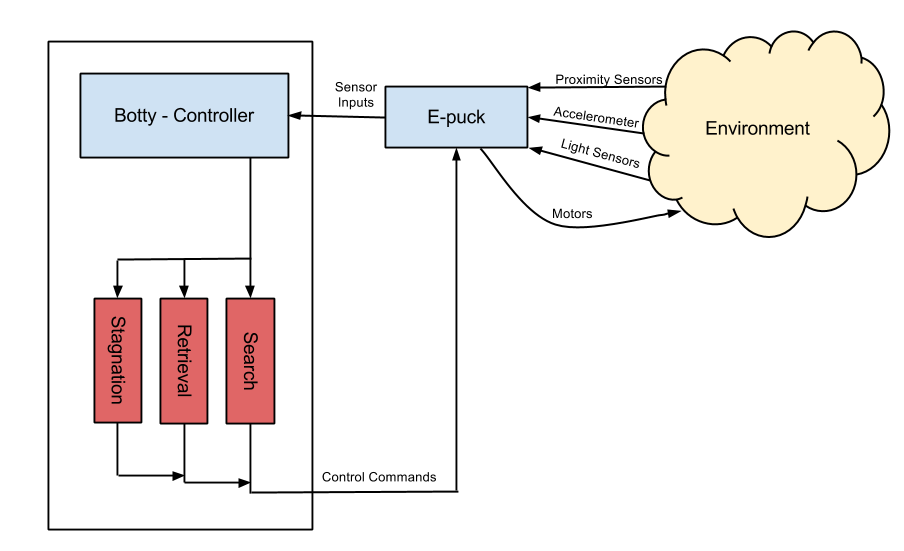
\includegraphics[width=0.99\textwidth]{models/SubSym Proj 4 architecture.png}
  \caption{Controller architecture for Box Pushing Task.}
  \label{fig:architecture}
\end{figure}

\subsection{Resulting behavior}

\section{Possible improvements}
\label{sec:b1}

\section{Implementating and evaluating the improvements}
\label{sec:b2}


\end{document}
